\section{Conclusiones}

\noindent

%% ---------------------------------------------------------------------------
%% FASE 1: PREPARACIÓN DEL ENTORNO
%% ---------------------------------------------------------------------------

\subsection{Fase 1: Preparación del entorno}

\quad

\noindent
Pese a que en esta sección no se ha realizado ningún modelo, 
es importante destacar que la preparación del entorno ha sido un 
proceso fundamental para el desarrollo de la práctica.

\quad

\noindent
También es resulta interesante mencionar el proceso de creación de imágenes sintéticas que al final no se 
usaron. Con el proceso que realizó, se generó una imagen una imagen sintética para cada
imagen que tuviera 2 tipos de animales o más en la misma imagen y que la segunda clase no fuera de fish.
Siguiendo esta idea solo se generaron unas 24 imágenes nuevas, y debido a la poca aportación de imágenes de clases poco 
representadas, se decidió no incluirlas en el \textit{dataset} final. 

\quad

\noindent
El proceso se llevó a cabo seleccionando las imágenes candidatas y eliminando los 
píxeles correspondientes a la primera clase predominante. Esto implicaba reemplazar 
las áreas ocupadas por los animales de dicha clase con el color del fondo original. 
A partir de esta modificación, se generó una nueva imagen sintética en la que la clase 
predominante pasó a ser la segunda más representativa de la imagen original.

\quad

\noindent
Siguiendo esta línea, 
se produjeron aproximadamente 24 imágenes nuevas; sin embargo, dada la escasa producción 
de imágenes de clases menos frecuentes, se optó por no incluirlas en el \textit{dataset} final.

\quad

\noindent
Como aprendizaje fuera de estas imágenes sintéticas, se ha comprobado la utilidad de usar pipelines de
proceso de imágenes, para automatizar el proceso de preparación de datos para el entrenamiento de modelos.

%% ---------------------------------------------------------------------------
%% FASE 2: IMPLEMENTACIÓN EN MODO PRE-TRAIN
%% ---------------------------------------------------------------------------

\subsection{Fase 2: Implementación en modo Pre-Train}

\noindent
En esta seccion se ha implementado una red neuronal convolucional (CNN) y se han
ido generando diferentes modelos a partir de esta red. Se ha ido modificando la arquitectura de la red,
Teniendo así los siguientes resultados:


\begin{figure}[H]
    \centering
    \begin{tabular}{|c|c|c|c|c|c|}
        \hline
        \textbf{Modelo} & \textbf{Capas} & \textbf{LR Factor} & \textbf{LR Patience} & \textbf{Val Acc} & \textbf{Test Acc} \\ \hline
        1 & 4 & 0.20 & 5 & 0.7480 & 0.8730 \\ \hline
        2 & 3 & 0.10 & 3 & 0.7795 & 0.8254 \\ \hline
        3 & 5 & 0.30 & 8 & 0.7717 & 0.7460 \\ \hline
    \end{tabular}
    \caption{Comparación de Modelos}
\end{figure}

\begin{center}
    \textbf{Mejor Modelo: \#1}
\end{center}

\begin{itemize}
    \item \textbf{Capas Convolucionales:} 4
    \item \textbf{Factor de Reducción LR:} 0.2
    \item \textbf{Paciencia para Reducción LR:} 5
    \item \textbf{Mejor Época:} 18
    \item \textbf{Precisión de Validación:} 0.7480
    \item \textbf{Precisión de Prueba:} 0.8730
\end{itemize}

\quad

\noindent
Como se observa existe una diferencia entre la precisión de validación y la de prueba.
Hay que tener en cuenta sin embargo que la precisión de test (prueba) es tan alta porque
las imagenes del train son muy parecidas a las de test, ya que el dataset está hecho con imágenes
un mismo video. Eso puede significar que el modelo no generalize fuera de este video o similares.

\quad

\noindent
Como aprendizaje de esta fase, la limitación de calidad de las imágenes no tiene porqué afectar
de forma muy negativa al modelo, y por lo tanto es una prueba que puede ser útil realizar en muchos 
otros casos debido a su bajo coste computacional.
\quad

\begin{figure}[H]
    \centering
    \centering
    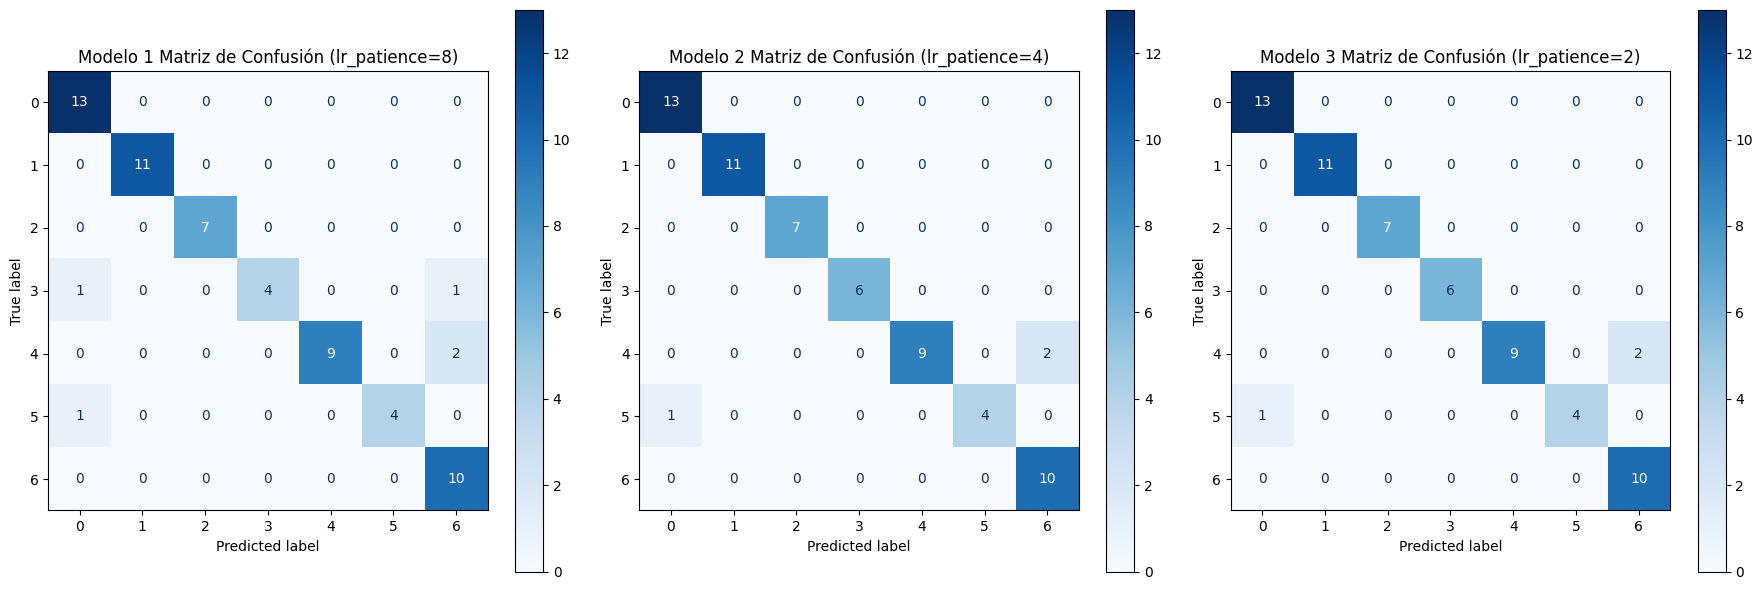
\includegraphics[width=\textwidth]{imagenes/confusion_matrix_a_quitar.png}
    \caption{Matrices de confusión.}
    \label{fig:confusion_matrix}
\end{figure}

\begin{figure}[H]
    \centering
    \centering
    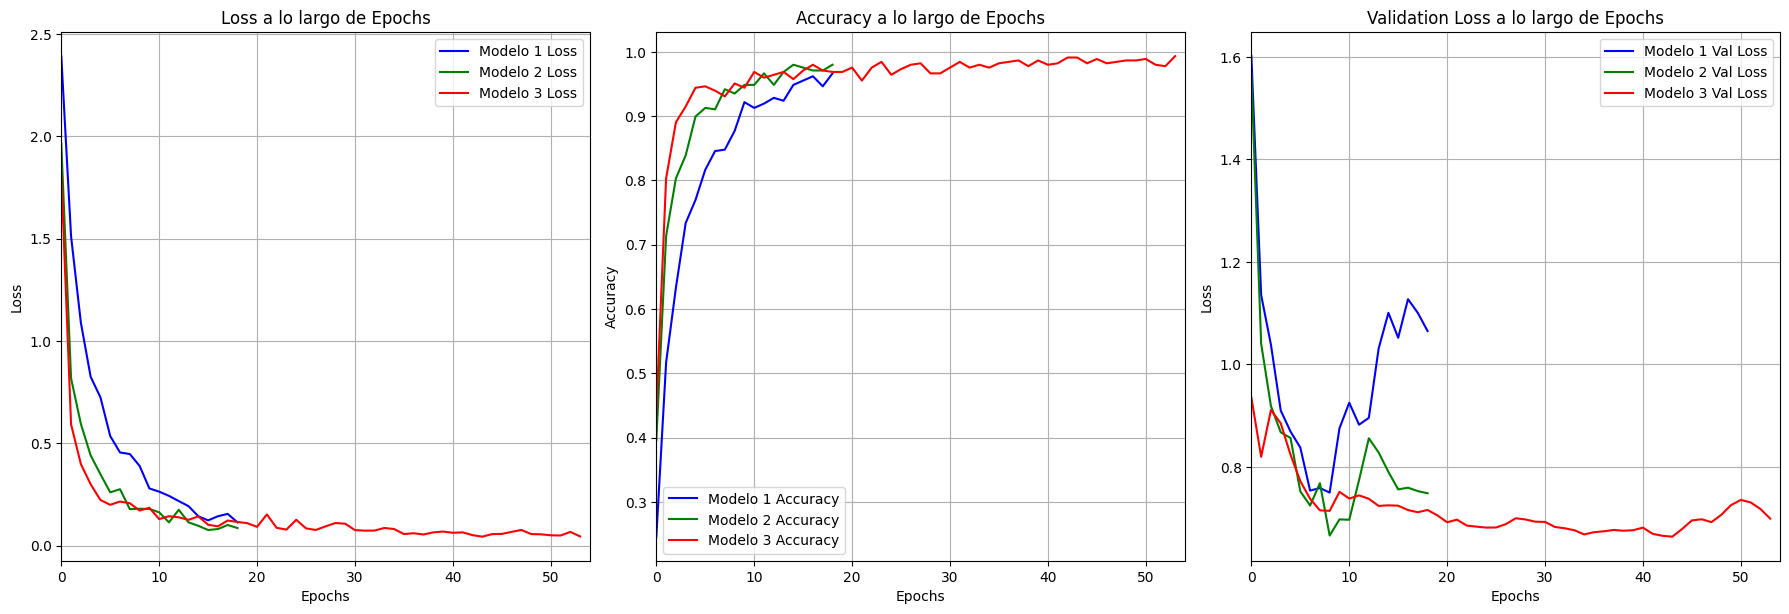
\includegraphics[width=\textwidth]{imagenes/loss_accuracy_validation_a_quitar.png}
    \caption{train\_loss, accuracy y val\_loss}
    \label{fig:loss_accuracy_validation}
\end{figure}

%% --------------------------------------------------------------------------
%% FASE 3: IMPLEMENTACIÓN EN MODO FINE-TUNNING
%% --------------------------------------------------------------------------

\subsection{Fase 3: Implementación en modo Fine-Tunning}

\noindent
En esta seccion se ha utilizado un modelo preentrenado como base (MobileNetV3Large) y se han
ido generando diferentes modelos modificando la tasa de learning rate variable definido por la paciencia. Para utilizar este modelo se ha eliminado su capa superior y solo se han entrado las 20 últimas capas, para adaptar el aprendizaje a nuestro problema y a la vez aprovechar los pesos preentrenados.
Teniendo así los siguientes resultados:


\begin{figure}[H]
    \centering
    \begin{tabular}{|c|c|c|c|c|c|}
        \hline
        \textbf{Modelo} & \textbf{LR Patience} & \textbf{Val Acc} & \textbf{Test Acc} \\ \hline
        MobileNetV3Large & 8 & 0.8346 & 0.9263 \\ \hline
        MobileNetV3Large & 4 & 0.8268 & 0.9367 \\ \hline
        MobileNetV3Large & 2 & 0.8346 & 0.9578 \\ \hline
    \end{tabular}
    \caption{Comparación de Modelos}
\end{figure}

\begin{center}
    \textbf{Mejor Modelo: \#3}
\end{center}

\begin{itemize}
    \item \textbf{Paciencia para Reducción LR:} 2
    \item \textbf{Mejor Época:} 36
    \item \textbf{Precisión de Validación:} 0.8346
    \item \textbf{Precisión de Prueba:} 0.9578
\end{itemize}

\quad

\noindent
Como aprendizaje de esta fase, encontramos la potencia de utilizar un modelo preentrenado como base, que puede ser reutilizado para nuestras propias tareas.
\quad

\begin{figure}[H]
    \centering
    \centering
    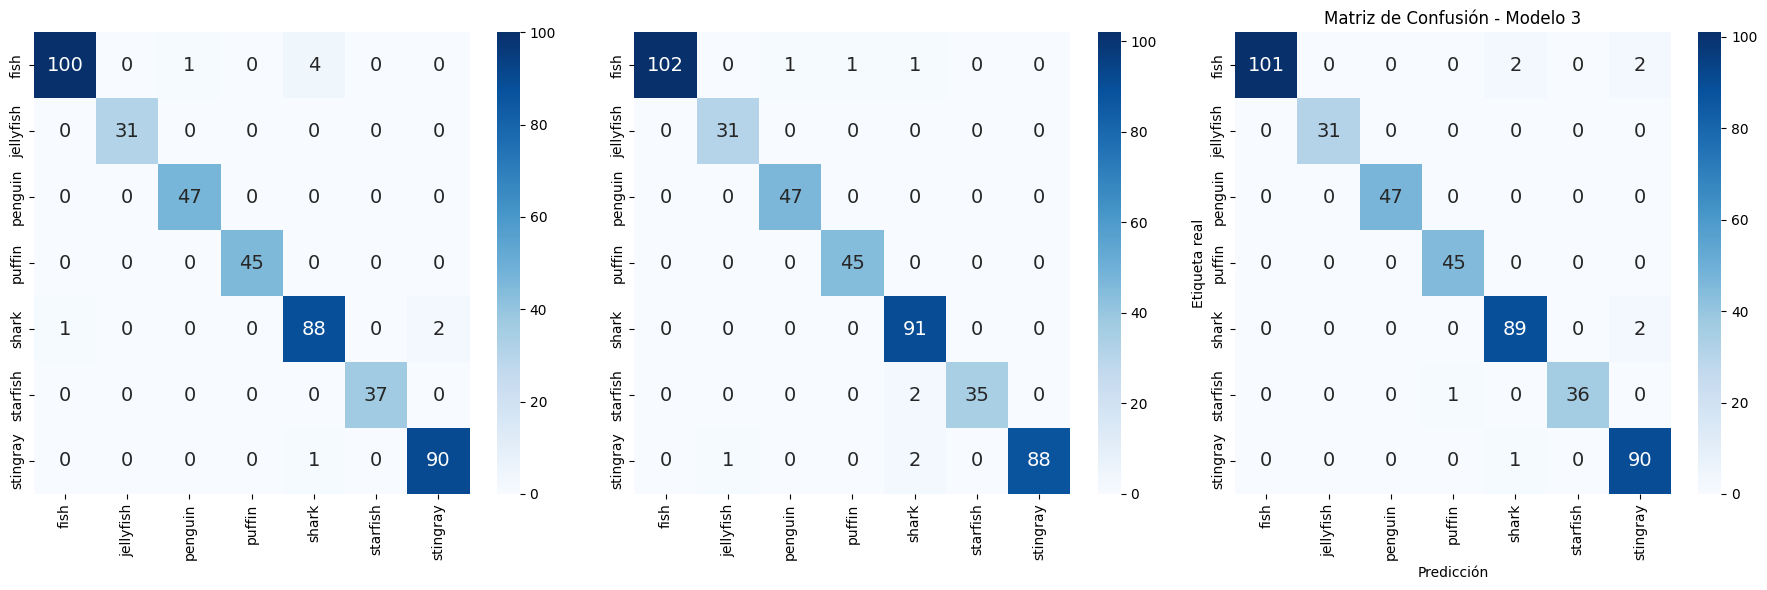
\includegraphics[width=\textwidth]{imagenes/train_fine2.png}
    \caption{Matrices de confusión entrenamiento.}
    \label{fig:confusion_matrix}
\end{figure}

\begin{figure}[H]
    \centering
    \centering
    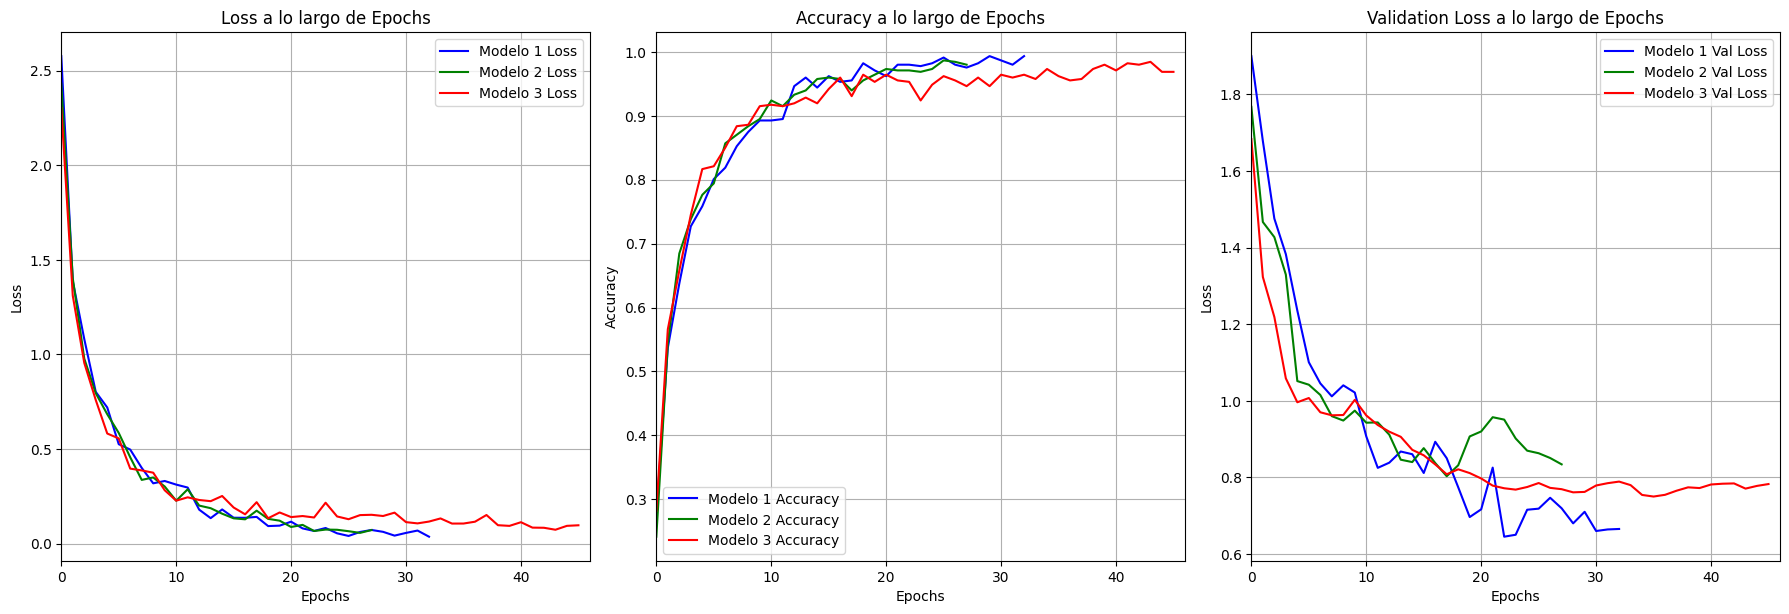
\includegraphics[width=\textwidth]{imagenes/train_fine.png}
    \caption{Matrices de confusión test + train\_loss, accuracy y val\_loss}
    \label{fig:loss_accuracy_validation}
\end{figure}
